% ---
% tags: [Scaling, Embedding, 参数规模]
% author: marshall
% excerpt:
% ---
\documentclass[11pt]{article}

\usepackage{fontspec}
\usepackage{xeCJK}
% macOS 上 SimSun 位于 Microsoft Word 内部；如需其它字体请修改下面路径
\setCJKmainfont[Path=/Applications/Microsoft Word.app/Contents/Resources/DFonts/, Extension=.ttc]{Simsun}

\usepackage[a4paper, margin=2.2cm]{geometry}
\linespread{1.3}
\setlength{\parskip}{0.3em}
\usepackage{amsmath, amssymb, amsthm}
\usepackage{graphicx}
% 本文图片统一放在与 .tex 同名的文件夹 latex/<slug>/ 中，直接用文件名引用即可
\graphicspath{{./}{2026-11-23-seed-papers-scale/}}
\usepackage{hyperref}
\hypersetup{colorlinks=true, linkcolor=blue, urlcolor=blue}

\title{串读两篇Seed论文，Scale参数的新视角}
\author{Marshall}

\begin{document}
\maketitle

本文介绍来自 Seed 团队的两篇论文，这两篇论文共同给出了一个 Scale 模型参数的新视角：

\begin{itemize}
  \item Over-Tokenized Transformer: Vocabulary is Generally Worth Scaling
  \item Virtual Width Networks
\end{itemize}

\section{Scale 参数的时候我们应该考虑什么？}

我们首先对模型里面的参数使用进行分类，大体可以分为以下三类：

\begin{itemize}
  \item dense GEMM：attention 的 QKV/O 投影和 FFN；
  \item 稀疏激活：MoE 部分；
  \item 稀疏查表：embedding。
\end{itemize}

我们从算力和显存两个方面去考虑，考虑 scale 相同单位的参数数量之后，这三类参数会带来的开销，有以下特征：扩第一类（dense GEMM）是直接加算力开销；扩第二类（稀疏激活）基本只加显存开销；扩第三类（稀疏查表）基本上访存和算力都不需要增加。

因此从这个角度出发，我们应该尽可能想办法将 scale 的参数塞进第三类参数，具体的开销可以参考下表：

\begin{table}[htbp]
  \centering
  \small
  \begin{tabular}{p{3.0cm}p{3.4cm}p{3.9cm}p{4.6cm}}
    \hline
    \textbf{扩展对象} & \textbf{加参数的位置} & \textbf{每 token 计算} & \textbf{主要工程代价} \\
    \hline
    hidden size / 层数 & dense GEMM & $O(D^2)$ 每层 & 算力、激活显存 \\
    \hline
    expert 数量（MoE） & sparse FFN & 只走 top-$k$ & all-to-all 路由 \\
    \hline
    输入词表（OE） & embedding 表的行数 & $O(1)$ 查表 & 参数显存、查表通信 \\
    \hline
    输出词表 & unembedding head & $O(V \cdot D)$ & 输出 GEMM、softmax \\
    \hline
  \end{tabular}
\end{table}

\section{Over-Encoding（OE）的动机与原理}

\subsection{两个视角来看 OE 的动机}

OE（Over-Tokenized Embedding）的设计动机可以从两个角度来理解。

\textbf{第一个角度：Embedding 层具有较高的参数扩展性价比。}

如第一章所述，对于 Transformer 来说，如果希望增加模型参数量，通常需要扩大隐藏层维度、增加网络层数，或者扩展 FFN 等模块。这些方式不仅会增加参数量，也会带来相应的计算量、显存占用以及通信开销。

但 Embedding 层有所不同。它本质上是一个查表操作（Lookup），模型根据 Token ID 从 Embedding 矩阵中取出对应的向量。增加 Embedding 的词表规模，虽然会增加参数存储量，但不会改变单次 Token 查表的计算复杂度。

换句话说，如果我们希望在增加模型参数量的同时，尽可能避免引入额外的计算负担，那么 Embedding 层就是一个非常值得考虑的扩展方向。

\textbf{第二个角度：传统 Embedding 存在一定的上下文表达局限。}

我们可以通过一个简单的例子来理解。

假设输入中存在一个 Token：「苹果」。它既可能出现在「吃苹果」这样的语境中，也可能出现在「维修苹果手机」这样的语境中。

在传统 Embedding 机制下，只要「苹果」对应的 Token ID 相同，那么它在输入阶段查表得到的 Embedding 向量就是完全相同的。

这可以理解为一种局部上下文表达上的局限：\textbf{单个 Token 拥有独立的向量表示，但相邻 Token 之间的组合关系，并没有直接体现在 Embedding 查表结果中。}

而 OE 希望解决的正是这个问题。它通过引入更丰富的 n-gram Embedding，让模型在输入阶段就能够感知局部 Token 组合。对于「苹果」来说，在「吃苹果」和「维修苹果手机」这两种语境中，模型可以查到不同的局部组合 Embedding，从而获得更加丰富的初始表示。

\subsection{OE 的原理}

\subsubsection{n-gram 和多路 embedding}

承接上一章，所谓局部性，可以引入 n-gram 这个概念，我们把连续 n 个 token 组成的片段当成一个整体单元：

\begin{itemize}
  \item $n=1$ 是单个 token 本身；
  \item $n=2$ 是相邻两个 token 的组合；
  \item $n=3$ 是相邻三个 token 的组合；
  \item 以此类推……
\end{itemize}

对于这些不同的 token 组合，我们都可以用扩展的额外的 embedding 词表进行表示。OE 的基本思路是：扩展 Embedding 层，为不同长度的 n-gram 引入额外的词表，并通过多路查表获取对应的向量表示。

整体结构可以理解为：同一个 Token Sequence 分别经过第 1 级、第 2 级……第 N 级的词表查找，各自得到 Embedding 向量，再分别经过线性投影，最后融合得到最终表示。

\begin{figure}[htbp]
  \centering
  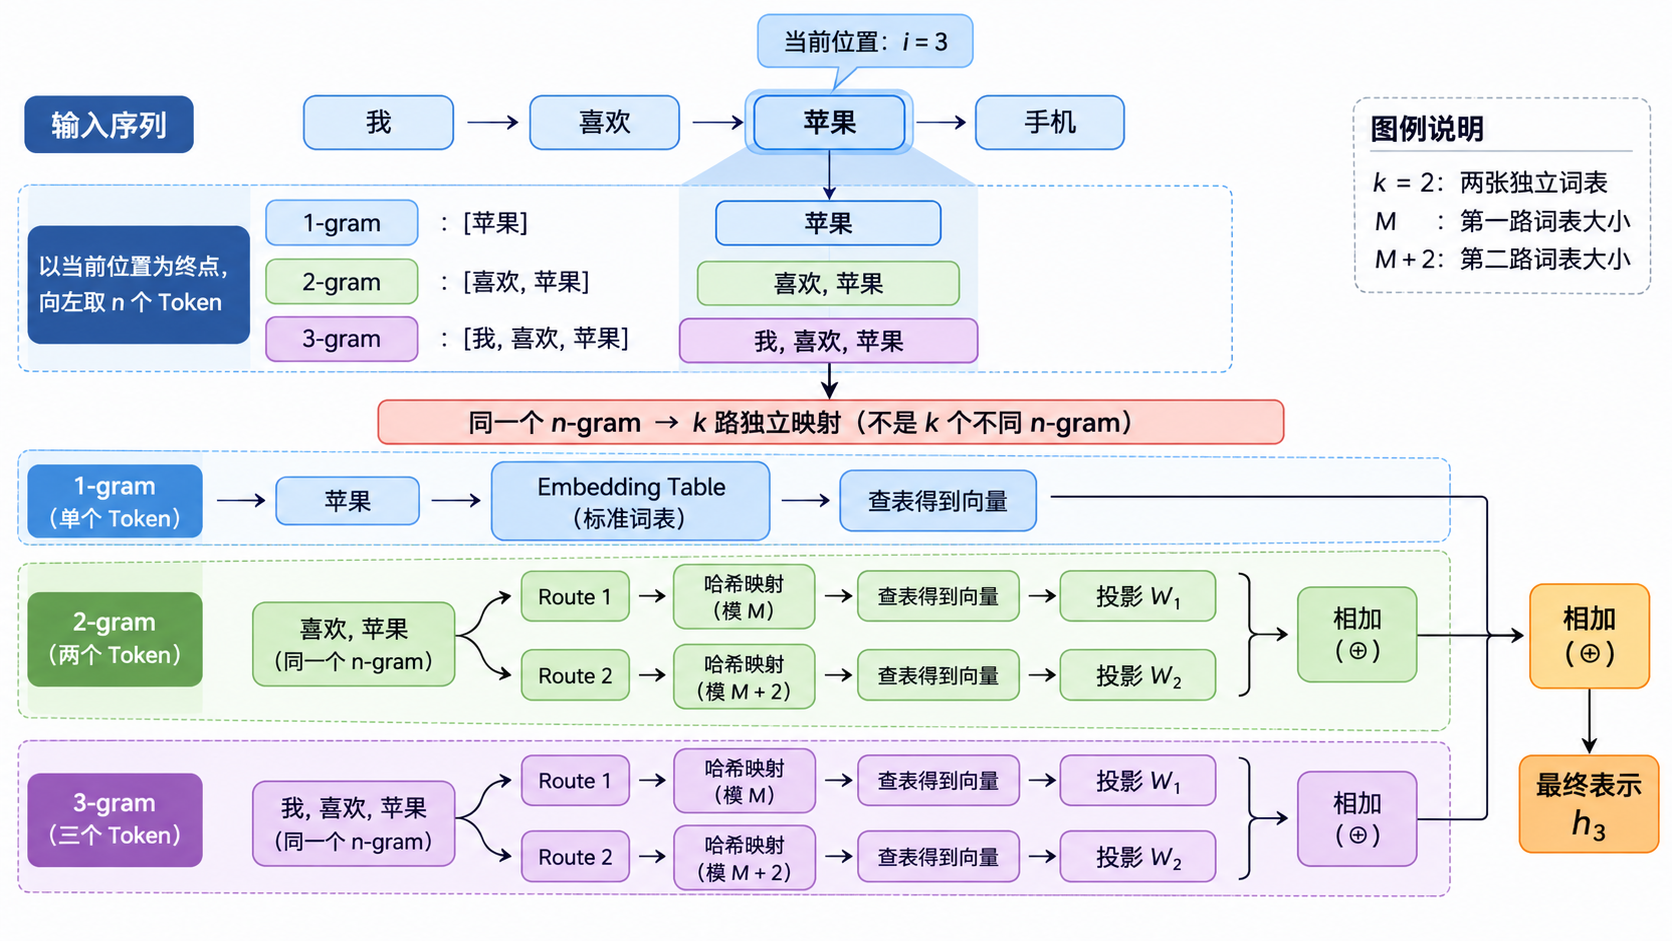
\includegraphics[width=0.8\textwidth]{oe-embedding.png}
  \caption{OE 的多路 n-gram embedding 结构}
  \label{fig:oe-embedding}
\end{figure}

\subsubsection{多路 embedding 的映射算法}

这里我们还需要补充一个细节，对于不同的 token 组合，扩展的多路词表是怎么来进行词表映射的呢？对于原生的标准词表我们很好理解，独立的 token ID 在词表里面唯一对应一个词向量表示，例如「苹果」对应 Token ID = 56，那么模型就直接通过 \texttt{Embedding[56]} 取出它的向量表示。

但是，对于 OE 扩展出来的 n-gram 词表，n-gram 的组合数量会随着长度迅速增长。假设原始词表大小为 $V$，那么理论上：

\begin{itemize}
  \item 1-gram：$V$ 种组合；
  \item 2-gram：$V^2$ 种组合；
  \item 3-gram：$V^3$ 种组合；
  \item n-gram：$V^n$ 种组合。
\end{itemize}

可想而知如果构建一个遍历所有组合的词表是不现实的，因此，OE 采用了一种基于整数编码和取模的映射方式。

\textbf{第一步：将连续 Token 组合编码成一个整数}

假设原始词表大小为 $V$，每个 Token 都有自己的 ID。对于一个 n-gram，OE 将其中的 Token ID 看作一个以 $V$ 为基数的数，编码为：
\[
  f(z_1,z_2,\ldots,z_n)=\sum_{j=1}^{n}z_j V^{j-1}
\]
例如，假设：

\begin{table}[htbp]
  \centering
  \small
  \begin{tabular}{p{4.0cm}p{4.0cm}}
    \hline
    \textbf{Token} & \textbf{Token ID} \\
    \hline
    我 & 12 \\
    喜欢 & 34 \\
    苹果 & 56 \\
    \hline
  \end{tabular}
\end{table}

那么，以「苹果」为当前位置，编码结果为：

\begin{table}[htbp]
  \centering
  \small
  \begin{tabular}{p{4.0cm}p{5.0cm}p{6.0cm}}
    \hline
    \textbf{n-gram} & \textbf{Token 组合} & \textbf{编码} \\
    \hline
    2-gram & [苹果, 喜欢] & $56 + 34 \times V$ \\
    \hline
    3-gram & [苹果, 喜欢, 我] & $56 + 34 \times V + 12 \times V^2$ \\
    \hline
  \end{tabular}
\end{table}

这样，不同的 Token 组合就可以被编码为不同的整数。

\textbf{第二步：通过取模，将组合映射到有限大小的 Embedding 表}

虽然上述整数编码可以区分不同的 n-gram 组合，但直接建立完整的 $V^n$ 大小的 Embedding 表仍然不现实。

OE 的做法是预先设置一个可配置的词表大小 $m$，然后对编码结果取模：
\[
  \operatorname{Index}(z_1,\ldots,z_n)=f(z_1,\ldots,z_n)\bmod m
\]
例如：

\begin{table}[htbp]
  \centering
  \small
  \begin{tabular}{p{6.0cm}p{5.0cm}}
    \hline
    \textbf{项目} & \textbf{数值} \\
    \hline
    原始 n-gram 编码 & 123456789 \\
    Embedding 表大小 & $m=10000$ \\
    最终查表索引 & $123456789 \bmod 10000 = 6789$ \\
    \hline
  \end{tabular}
\end{table}

于是，这个 n-gram 就映射到了 Embedding 矩阵的第 6789 行。

这里有一个重要的区别：\textbf{不同的 n-gram 组合可能映射到同一个索引。}

也就是说，OE 并不保证每个 n-gram 都有独立的 Embedding 向量，而是允许不同组合共享同一行参数。这本质上是一种哈希映射（Hashing），通过接受一定程度的碰撞，换取有限的参数规模。

\textbf{第三步：为什么还需要多路词表？}

如果只有一张大小为 $m$ 的 Embedding 表，那么所有 n-gram 都使用相同的取模规则，部分组合可能持续发生碰撞。

为此，OE 进一步引入多路 Embedding。假设有 $k=2$ 路，那么同一个 n-gram 编码会分别映射到两张大小不同的词表：
\[
  I_1=f(z_1,\ldots,z_n)\bmod m
\]
\[
  I_2=f(z_1,\ldots,z_n)\bmod (m+2)
\]
例如：

\begin{table}[htbp]
  \centering
  \small
  \begin{tabular}{p{4.0cm}p{5.0cm}p{6.0cm}}
    \hline
    \textbf{路径} & \textbf{词表大小} & \textbf{取模结果} \\
    \hline
    第 1 路 & $m=10000$ & $123456789 \bmod 10000 = 6789$ \\
    \hline
    第 2 路 & $m+2=10002$ & $123456789 \bmod 10002 = 6783$ \\
    \hline
  \end{tabular}
\end{table}

两路分别从自己的 Embedding 表中查出向量，再通过对应的投影矩阵映射到模型隐藏维度。

这样，即使两个 n-gram 在第一路中发生碰撞，也不意味着它们在第二路中一定发生碰撞。

需要注意的是，这里的多路并不是采用不同的 n-gram 组合，而是对同一个 n-gram 使用不同的词表大小进行映射。

\textbf{总结一下：}标准 Embedding 是 Token ID → Embedding；OE 扩展的 n-gram Embedding 则是 Token 组合 → 整数编码 → 取模映射 → Embedding。再通过多路映射和低秩投影，进一步增强局部组合的表示能力。

\subsubsection{如何融合 embedding}

简单来说，我们先取普通 token embedding，再把各路 n-gram embedding 投影后相加，最后按分支数量缩放：
\[
  h_t=\frac{e_{\mathrm{word},t}+\sum_{n=2}^{N}\sum_{j=1}^{k}P_{n,j}(e_{n,j,t})}{1+k(N-1)}
\]
其中 $N$ 是 n-gram 的最大长度，$k$ 指词表的“路数”（即同一个 n-gram 用 $k$ 张不同大小的词表并行查表的分支条数），$e_{n,j,t}$ 是第 $j$ 路查表得到的 n-gram 向量，$P_{n,j}$ 是这一路专属的低秩投影矩阵。

回到前面「我、喜欢、苹果、手机」这个例子，「苹果」这个位置的完整流程就是：「苹果」的普通 embedding，加上两路 [苹果, 喜欢] 的小向量投影结果，再加上两路 [苹果, 喜欢, 我] 的小向量投影结果，最后按总分支数缩放，得到「苹果」这个位置的 $D$ 维模型输入。

所以，OE 扩大的是可供查询的输入参数和组合特征，\textbf{最终进入 Transformer 的向量仍然是 $D$ 维}，后续 backbone 不需要因此一起变宽。

\section{VWN 的动机与原理}

\subsection{VWN 的动机}

回过头再看 OE 的做法，会觉得它有些别扭。我们想扩充参数量，最直观的动作就是把词表做大。OE 也确实扩大了输入词表，但为了让最终输出的词向量仍与 backbone 保持同样的宽度 $D$，还需要额外引入一套映射算法。

那么，有没有一种方式可以更直接地 scale 参数？比如让整个网络一起变宽，同时又不带来太多额外开销？

VWN（Virtual Width Networks）正是顺着这个思路提出的，其对两个概念进行了分离：

\begin{itemize}
  \item \textbf{Backbone Width}：Transformer 内部实际参与 Attention、FFN 等计算的隐藏维度，保持不变；
  \item \textbf{Virtual Width}：Token Embedding 以及中间隐藏表示所使用的扩展维度，可以在原有基础上进一步扩大。
\end{itemize}

这样一来，我们就能够在不显著增加 Backbone 计算量的前提下，为模型提供更大的表示空间。

\subsection{VWN 的原理}

VWN 的做法可以拆成两步：先用 Over-Width Embedding 把 Token 的表示做宽，再用 GHC 在宽表示与窄 Backbone 之间来回转换。

\subsubsection{Over-Width Embedding：构造更宽的输入表示}

Over-Width Embedding 将输入的词表扩大，我们假设原始词表的维度是 $D$，那么新的扩大后的词表大小就是 $D'$，扩大比例可以记为 $r$：
\[
  D'=rD
\]
比方说，$D=8$、$r=2$，那么入口向量就是 16 维。构造宽输入有两种常见方式：

\begin{itemize}
  \item \textbf{直接使用宽 embedding 表}：将表从 $V\times D$ 扩为 $V\times D'$，每个 token ID 直接查出一个 $D'$ 维向量。$V$ 是普通词表大小。
  \item \textbf{基础 embedding 加共享投影}：保留 $V\times D$ 的基础表，先查出 $D$ 维向量，再用所有 token 共享的 $W_{\mathrm{expand}}$ 将其映射到 $D'$ 维：
  \[
    e_{\mathrm{wide}}=W_{\mathrm{expand}}e_{\mathrm{base}}
  \]
\end{itemize}

第二种方式相当于对宽表做低秩参数化，可以降低表的存储成本。

如果希望补充局部组合信息，也可以将前文 OE 的特征与普通 embedding 融合后，构造宽输入。OE 提供输入增强，Over-Width Embedding 提供宽表示，两者可以组合。

接下来的问题是：$D'$ 维状态如何送入只接收 $D$ 维输入的子层，又如何接收子层的计算结果？VWN 通过下面的 GHC 完成这两种宽度之间的交互。

\begin{figure}[htbp]
  \centering
  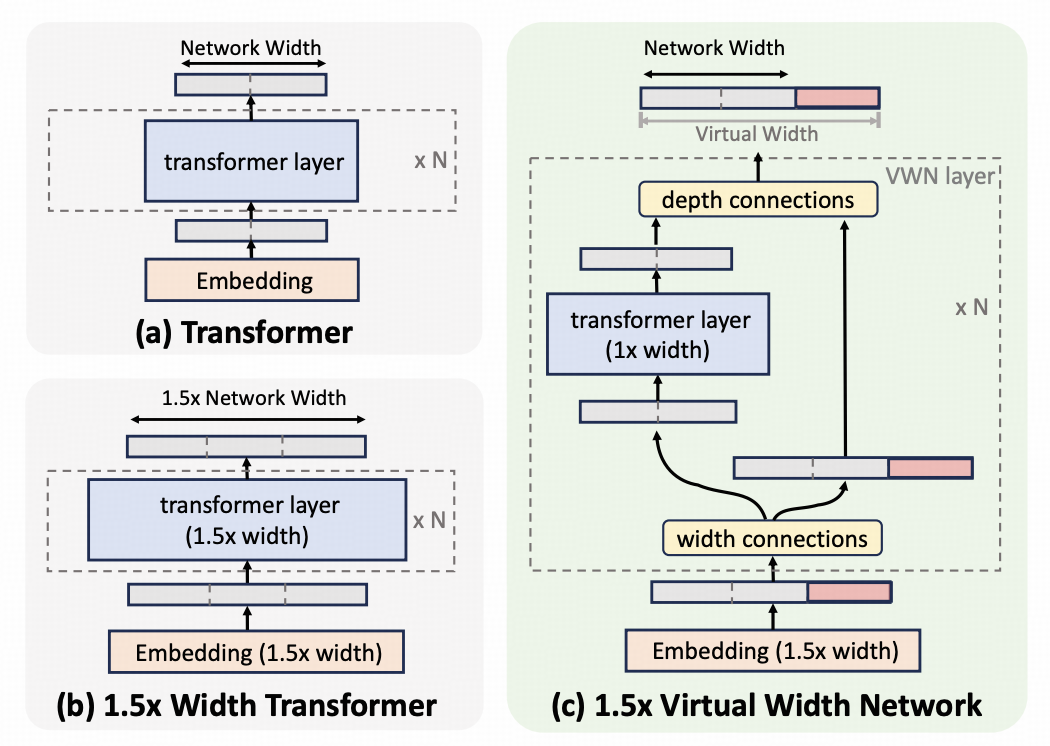
\includegraphics[width=0.8\textwidth]{ghc.png}
  \caption{GHC 在宽表示与窄 backbone 之间的映射}
  \label{fig:ghc}
\end{figure}

\subsubsection{Generalized Hyper-Connections（GHC）：在 D 维与 D' 维之间映射}

简单来说 GHC 实现的就是两个映射：从 $D'$ 维映射到 $D$ 维作为 transformer backbone 的输入；transformer backbone 计算完成后，将输出的 $D$ 维再映射回 $D'$ 参数空间。

为了下面的算法解释，我们引入两个字母 $m$ 和 $n$：将 $D$ 维分为 $m$ 组，将 $D'$ 维分为 $n$ 组，使两者每组的宽度相同。用 $d_b$ 表示每组宽度，$r$ 表示 $D'$ 相对于 $D$ 的扩宽倍数：
\[
  d_b=\frac{D}{m}=\frac{D'}{n},\qquad r=\frac{n}{m}
\]
我们以 $D=8$、$D'=16$ 为例，选择 $m=2$、$n=4$：

\begin{figure}[htbp]
  \centering
  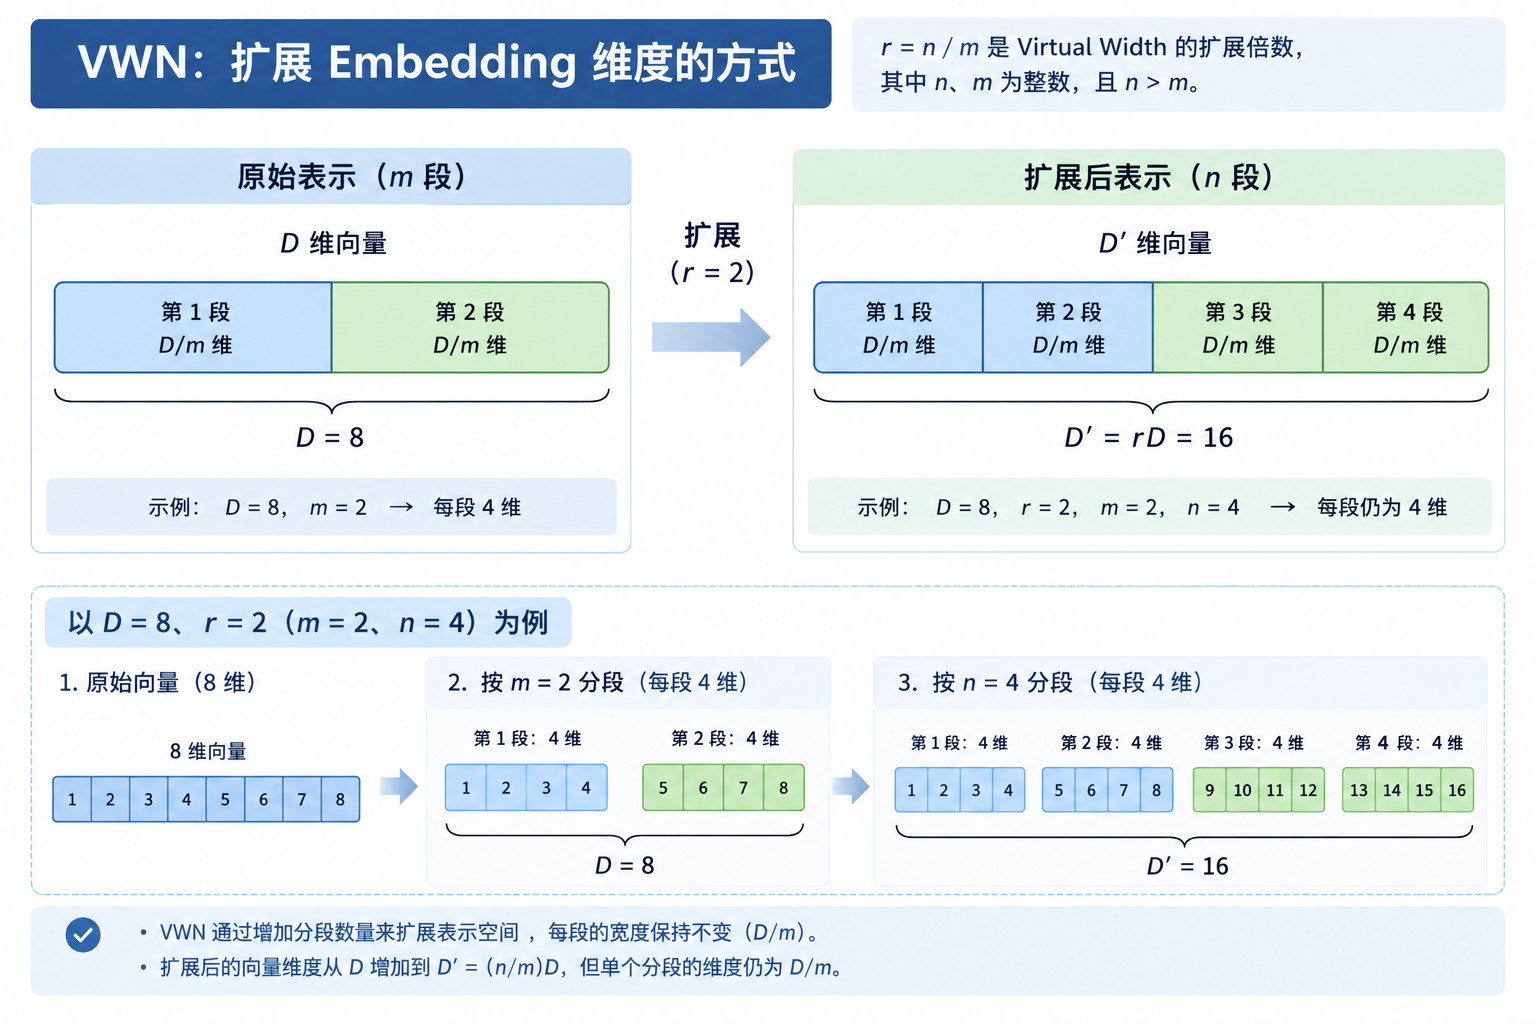
\includegraphics[width=0.8\textwidth]{ghc-example.png}
  \caption{$D=8$、$D'=16$ 时的 GHC 分组示意}
  \label{fig:ghc-example}
\end{figure}

\textbf{第一步：将 $D'$ 维表示映射到 $D$ 维，作为 Attention 或 FFN 的输入。}

将 16 维表示拆成四个 4 维向量 $h_1, h_2, h_3, h_4$，排成矩阵 $H$：
\[
  H=[h_1;h_2;h_3;h_4]\in\mathbb{R}^{4\times4}
\]
$A_{\mathrm{in}}$ 是系数矩阵，形状为 $4\times2$。通过以下操作，我们就可以得到 Attention 或 FFN 的输入：
\[
  X=A_{\mathrm{in}}^\top H\in\mathbb{R}^{2\times4},\qquad x=\operatorname{flatten}(X)\in\mathbb{R}^{8}
\]
\begin{verbatim}
h1, h2, h3, h4 = H
x1 = A_in[0,0]*h1 + A_in[1,0]*h2 + A_in[2,0]*h3 + A_in[3,0]*h4
x2 = A_in[0,1]*h1 + A_in[1,1]*h2 + A_in[2,1]*h3 + A_in[3,1]*h4
X = torch.stack([x1, x2])   # [2, 4]
x = X.flatten(-2)           # [8], map 16 -> 8
\end{verbatim}

$A_{\mathrm{res}}$ 是用于残差相加的权重矩阵，形状为 $n\times n$。它对原来的四组做加权组合，结果记为 $R$，仍然是 16 维。将 $A_{\mathrm{in}}$、$A_{\mathrm{res}}$ 按列拼接，记为矩阵 $A$：
\[
  A=[A_{\mathrm{in}},A_{\mathrm{res}}],\qquad X=A_{\mathrm{in}}^\top H,\qquad R=A_{\mathrm{res}}^\top H
\]
\begin{verbatim}
A_in = A[:, :m]   # [n, m] = [4, 2]
A_res = A[:, m:]  # [n, n] = [4, 4]
X = A_in.T @ H    # [2, 4], 2 groups, 8 dims
R = A_res.T @ H   # [4, 4], 4 groups, 16 dims
\end{verbatim}

\textbf{第二步：在 $D$ 维完成 Attention 或 FFN 计算。}

用 $T$ 表示 Attention 或 FFN。将 $X$ 的两组拼成 8 维向量 $x$，送入 $T$；输出记为 $y$，仍然是 8 维，再拆成两组，记为矩阵 $Y$。这里其实就是一个标准的 transformer 计算模块，Attention 或 FFN 的计算维度仍然是 $D$：
\[
  Y=\operatorname{reshape}_{m\times d_b}\!\left(T(\operatorname{flatten}(X))\right)
\]
\begin{verbatim}
# T denotes Attention or FFN; batch and token dims omitted
x = X.flatten(-2)      # [2, 4] -> [8]
y = T(x)               # [8] -> [8]
Y = y.reshape(m, d_b)  # [8] -> [2, 4]
\end{verbatim}

\textbf{第三步：将计算结果映射回 $D'$ 维。}

$B$ 是将 Attn/FFN 输出映射回宽表示的系数矩阵，形状为 $m\times n$。还记得我们上文提到的残差结果 $R$ 吗？在这里我们就会用到来生成新的 $D'$ 维宽表示：
\[
  H_{\mathrm{new}}=R+B^\top Y
\]
\begin{verbatim}
update = B.T @ Y  # combined result: [4, 2] @ [2, 4] -> [4, 4]
H_new = R + update
# i is the group index (0, 1, 2, 3):
# H_new[i] = R[i] + B[0,i]*Y[0] + B[1,i]*Y[1]
\end{verbatim}

\textbf{$m$、$n$、$A$、$B$ 分别怎么设置？}

$m$、$n$ 是分组数（超参数），$A$、$B$ 由训练学习。静态权重初始化如下，代码中的 \_init 表示初始值：
\[
  D=m\,d_b,\qquad D'=n\,d_b
\]
\begin{verbatim}
A_in_init = torch.zeros(n, m)
A_in_init[:m] = torch.eye(m)  # init: use first m groups as input
A_res_init = torch.eye(n)     # init: keep all n groups
B_init = torch.zeros(m, n)
j = torch.arange(n)           # j is the index of n output groups
B_init[j % m, j] = 1.0        # init: cyclic assignment
\end{verbatim}

本例 $m=2$、$n=4$，初始化时就是：
\[
  X=[h_1;h_2],\qquad R=H,\qquad H_{\mathrm{new}}=[h_1+y_1;\ h_2+y_2;\ h_3+y_1;\ h_4+y_2]
\]
这些 0、1 只是初始值，训练后可以变成不同的权重；按相同位置组合、组内共用权重的计算规则保持不变。

\textbf{动态 GHC：让组合系数随隐藏状态变化}

把前面由训练学到的系数记作 $A_{\mathrm{static}}$、$B_{\mathrm{static}}$。Dynamic GHC 根据当前 $H$ 生成一份调整量叠加其上，让不同 token 可以用不同的组合系数：
\[
  \bar H=\operatorname{norm}(H),\qquad \tau=\sqrt{d_b}
\]
\[
  \Delta A=S_A\odot\tanh\!\left(\frac{\bar H W_A}{\tau}\right),\qquad A=A_{\mathrm{static}}+\Delta A
\]
\[
  \Delta B=S_B\odot\tanh\!\left(\frac{\bar H W_B}{\tau}\right)^{\top},\qquad B=B_{\mathrm{static}}+\Delta B
\]
其中 $\Delta A\in\mathbb{R}^{n\times(m+n)}$、$\Delta B\in\mathbb{R}^{m\times n}$ 是逐 token 的调整量，$S_A$、$S_B$ 与它们同形、控制调整幅度并初始化为 1，$W_A\in\mathbb{R}^{d_b\times(m+n)}$、$W_B\in\mathbb{R}^{d_b\times m}$ 是生成调整量的两个投影矩阵。

\begin{verbatim}
H_norm = norm(H)                                # [n, d_b]
tau = math.sqrt(d_b)                            # sqrt of group width
dA = S_A * torch.tanh(H_norm @ W_A / tau)       # [n, m+n]
dB = S_B * torch.tanh((H_norm @ W_B) / tau).T   # [m, n]
A = A_static + dA
B = B_static + dB
\end{verbatim}

不同 token 因此可以采用不同的组合系数，矩阵形状与计算流程保持不变。

\textbf{算法思想：}

我们来简单阐述一下整个 GHC 算法流程设计的思想：$A$ 负责把宽表示压成 $D$ 维输入，同时决定旧表示保留多少（残差加回去）；$B$ 负责把 $D$ 维结果写回 $D'$ 维。具体说，$A$ 的前 $m$ 列压出 Attention/FFN 的输入，后 $n$ 列给出残差 $R$；$B$ 把计算结果分配到各组，再与 $R$ 相加。

静态系数对所有 token 相同，但不同 token 该压出什么信息、该保留哪些旧表示并不一样。让 $A$、$B$ 由当前 $H$ 生成，就是把这套组合方式变成随内容变化的。

\subsubsection{开销推算}

Attention/FFN 仍按 $D$ 维计算，VWN 的新增开销主要来自动态系数生成、组间组合，以及 $D'$ 维表示的存储和读写。下面按每个 token、一个 Attention 或 FFN 的一套动态 GHC 计算，一次乘加计 2 FLOPs，每组宽度 $d_b=D/m$：

\begin{table}[htbp]
  \centering
  \small
  \begin{tabular}{p{5.4cm}p{5.0cm}p{4.0cm}}
    \hline
    \textbf{新增操作} & \textbf{主要 FLOPs} & \textbf{$m=2$、$n=4$ 时} \\
    \hline
    宽状态归一化 & $4(n/m)D$ & $8D$ \\
    \hline
    生成动态 A、B & $2(2m+n)(n/m)D$ & $32D$ \\
    \hline
    构造输入 X 和残差 R & $2(m+n)(n/m)D$ & $24D$ \\
    \hline
    将子层结果映射回宽表示 & $2nD$ & $8D$ \\
    \hline
    合计 & 上述四项之和 & $72D$ \\
    \hline
  \end{tabular}
\end{table}

动态系数生成对应前文的两个小线性投影，主要计算量为：
\[
  2n d_b (m+n)+2n d_b m=2(2m+n)(n/m)D
\]
本例 $m=2$、$n=4$，单个子层的动态 GHC 主要计算合计 $72D$；一个 block 的 Attention 和 FFN 各使用一套，共计 $144D$。

\textbf{与直接加宽 backbone 对比：}将表示宽度都取为 $D' = 2D$。以标准多头 Attention 的四个 $D\times D$ 投影，以及非门控 FFN（$D\to4D\to D$）为例，原 block 每 token 的线性投影 FLOPs 为 $8D^2+16D^2=24D^2$，矩阵参数量为 $12D^2$。直接将 backbone 加宽到 $2D$，这些投影的参数和 FLOPs 都变为 4 倍，新增 FLOPs 为 $72D^2$，即基线的 300\%；VWN 保持这些投影的维度不变，新增动态 GHC 的主要计算为 $144D$。

下面比较不同 $D$ 下的新增开销，计算量单位为 MFLOPs（百万 FLOPs）；占比分母统一为原 block 的线性投影 FLOPs：
\[
  \text{VWN 新增计算占比}=\frac{144D}{24D^2}=\frac{6}{D}
\]
\begin{table}[htbp]
  \centering
  \small
  \begin{tabular}{p{1.6cm}p{2.8cm}p{3.6cm}p{3.0cm}p{3.0cm}}
    \hline
    $D$ & 基线 FLOPs & 直接加宽至 2D 的新增 FLOPs & VWN 新增 FLOPs & VWN 新增 / 基线 \\
    \hline
    1024 & 25.17 & 75.50 & 0.147 & 0.586\% \\
    \hline
    2048 & 100.66 & 301.99 & 0.295 & 0.293\% \\
    \hline
    4096 & 402.65 & 1207.96 & 0.590 & 0.146\% \\
    \hline
    8192 & 1610.61 & 4831.84 & 1.180 & 0.073\% \\
    \hline
  \end{tabular}
\end{table}

\begin{figure}[htbp]
  \centering
  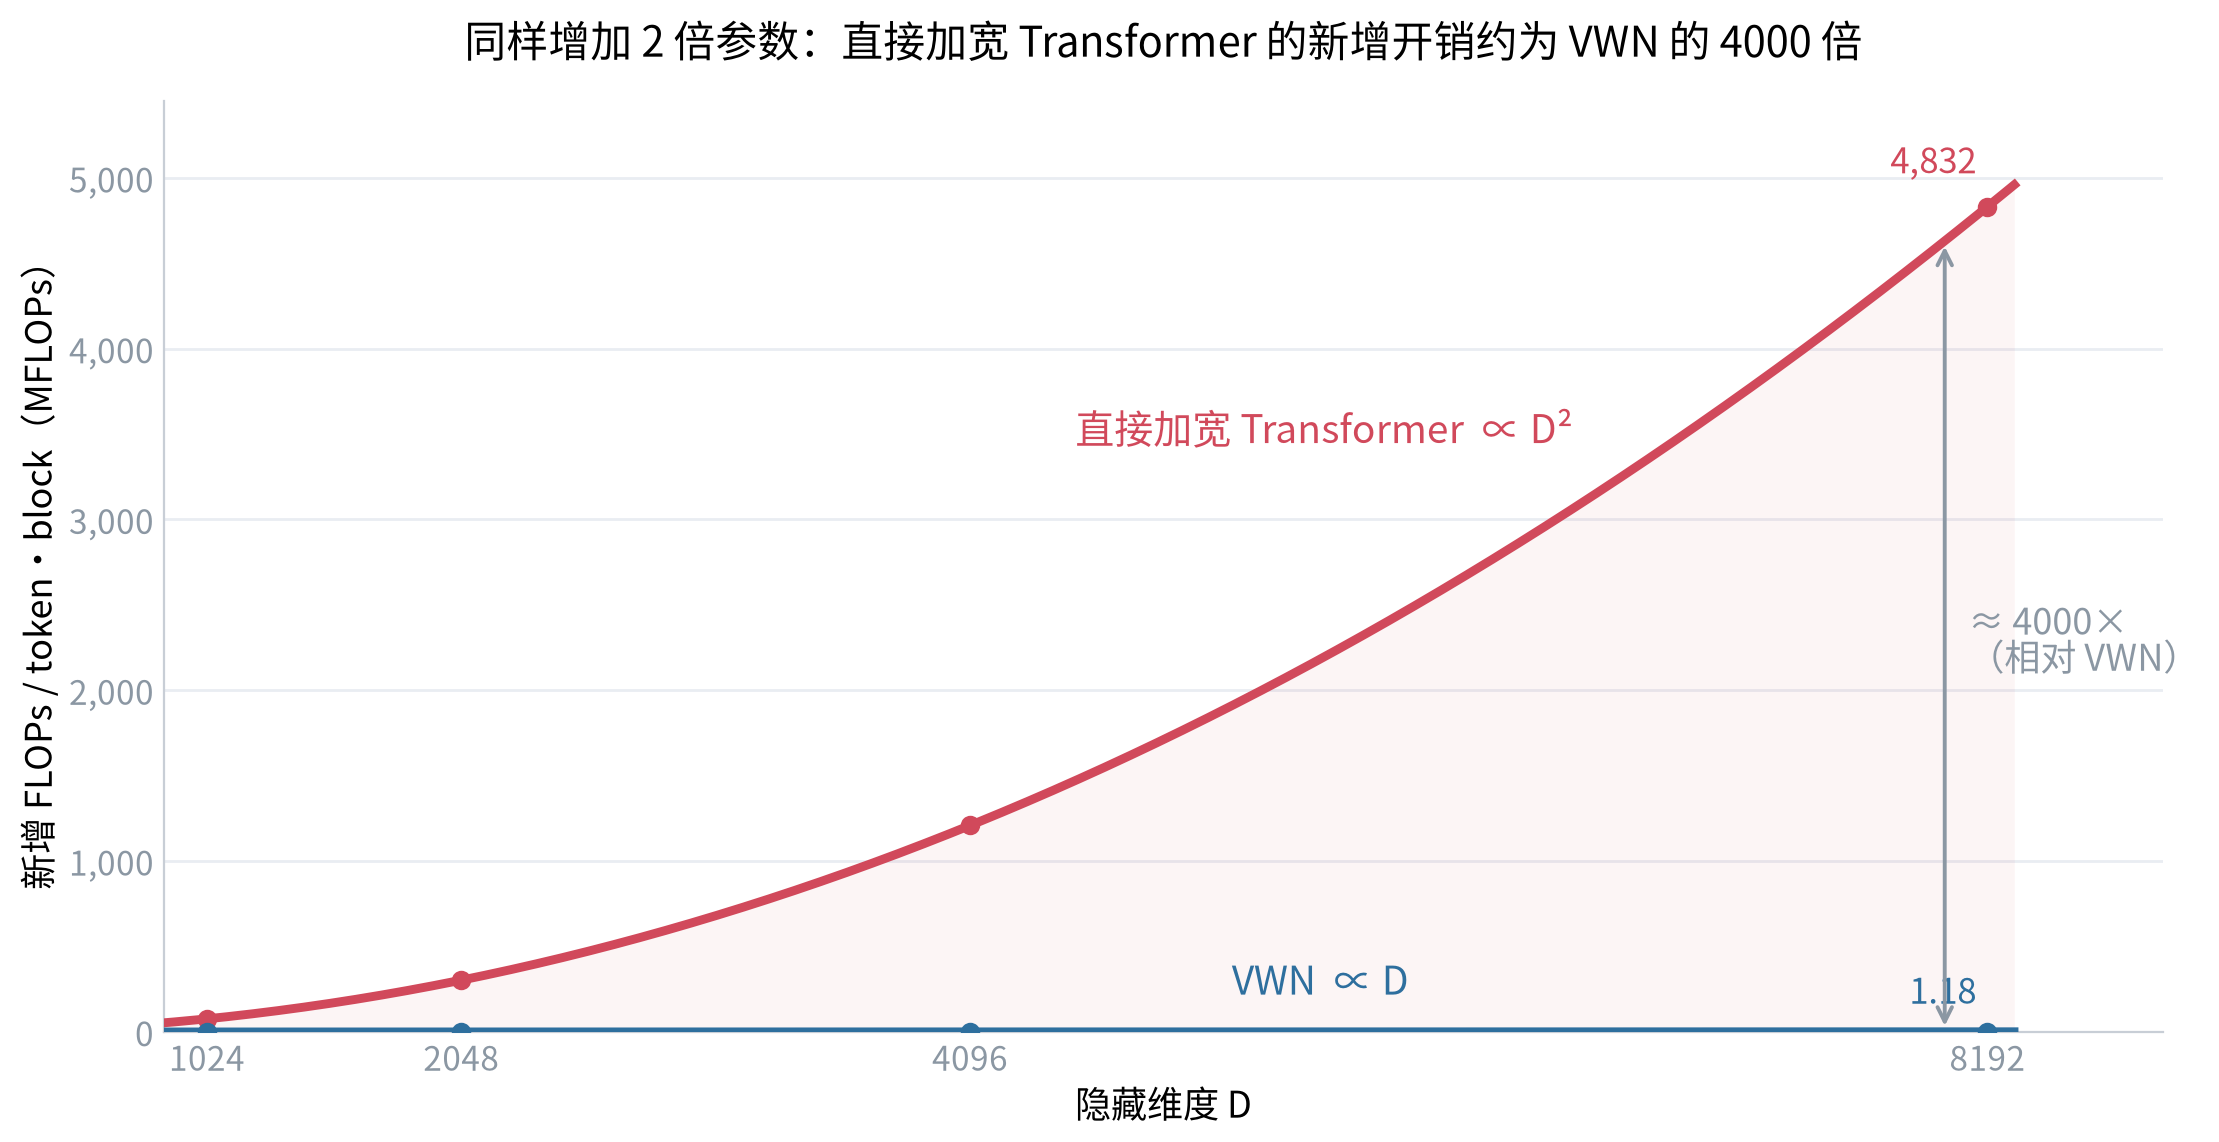
\includegraphics[width=0.75\textwidth]{vwn-flops.png}
  \caption{VWN 新增计算占比随 $D$ 的变化}
  \label{fig:vwn-flops}
\end{figure}

\textbf{显存：}直接将 embedding 表从 $V\times D$ 加宽为 $V\times D'$，参数量随宽度比例增长；采用基础表加共享升维投影时，则按基础表和投影矩阵计算。$D'$ 维中间表示也需要更多缓冲和训练激活存储，可以通过重计算减少保存量。


\end{document}
